\documentclass[a4paper,12pt]{report}
\usepackage{amsmath}
\usepackage[estonian]{babel}
\usepackage[bf]{caption}
\usepackage[top=2.54cm, bottom=2.54cm, left=3cm, right=2cm]{geometry}
\usepackage[utf8]{inputenc}
\usepackage{sectsty}
\usepackage[compact]{titlesec}
\usepackage{wrapfig}
\usepackage{graphicx}
\usepackage{subfig}
\usepackage{esvect}
\renewcommand{\vec}[1]{\vv{#1}}
\usepackage{listings}
\lstset{basicstyle=\footnotesize, language=C++, numbers=left, numberbychapter=false}
\chapterfont{\fontsize{16pt}{19pt}\sffamily}
\linespread{1.5	}
\renewcommand{\thechapter}{\arabic{chapter}.}
\renewcommand{\thesection}{\thechapter\arabic{section}.}
\renewcommand{\thesubsection}{\thesection\arabic{subsection}.}
\renewcommand{\thesubsubsection}{\thesubsection\arabic{subsubsection}.}
\renewcommand{\theequation}{\thechapter\arabic{equation}}
\renewcommand{\thefigure}{\thechapter\arabic{figure}}
\renewcommand{\lstlistlistingname}{Programmid}
\renewcommand{\lstlistingname}{Programm}

% et nad kaklema ei läheks
\usepackage[colorlinks=true]{hyperref}
\usepackage[tocbib]{apacite}

\pagestyle{empty}
\begin{document}
\begin{center}
Tallinna Reaalkool

\vfill

Kiirtejälitus\\
Uurimistöö

\vfill

\end{center}

\begin{raggedleft}

Andreas Ots

11a

Juhendaja: õp Inga Petuhhov

\end{raggedleft}

\vfill

\begin{center}

Tallinn 2011

\end{center}
\clearpage

\addtocontents{toc}{\protect\thispagestyle{empty}}
\tableofcontents
\listoffigures

\chapter*{Sissejuhatus}
\addcontentsline{toc}{chapter}{Sissejuhatus}
\thispagestyle{empty}
Kui kolmemõõtmeline arvutigraafika levima hakkas oli kaks võimalikku
algoritmi: rasteriseerimine ja kiirtejälitus. Rasteriseerimist on võimalik
realiseerida kasutades ainult täisarvude aritmeetikat, kiirtejälitust on
võimalik realiseerida ainult ujukomaaritmeetikat. Ujukomaaritmeetika oli
aeglane võrreldes täisarvude omaga, mis ei ole enam nii. 

Rasteriseerimine on liikunud üle ujukomaarvudele ja protsessori asemel
toimub joonistamine graafikakaardis, mille abil on võimalik joonistada
miljoneid kolmnurki kaadrisagedustel üle 30 kaadri sekundis koos erinevate
effektidega. Kiirtejälitusega on võimalik kasutada ära senist infrastruktuuri
ja saada realistlikum tulemus.

Uurimistöö eesmärgiks on luua ülevaade kiirtejälitusest ning olla aluseks
selle teema edasisel uurimisel.

Uurimistöö allikatena on kasutatud internetist kättesaadavaid selle ala
teaduslikke artikleid ja doktoritöid.

Uurimistöö koosneb ühest teoreetilise osa peatükist, milles on kuus
alampeatükki. Praktiline osa puudub. Lisa \ref{chap:download} sisaldab
uurimistöö raames valminud kiirtejälitaja kompileerimiseks vajalikku
informatsiooni.

\chapter{Kiirtejälitus}
\section{Kiirtejälituse mõiste}
Järgnev lõik pärineb Eesti Standardikeskuse standardist EVS-ISO/IEC~2382-13:1998:
\begin{quote}
Kiirtejälitus --- Vaatleja silmast stseeni objektideni kulgevate
kujuteldavate valguskiirte jälitusel põhinev meetod stseeni nende osade
määramiseks, mis tuleb kuvada saadaval pildil.\cite{ISO:2382-13}
\end{quote}

Kiirtejälitus pakub praeguseni teadaolevatest ilmestusmeetoditest kõige
realistlikumat tulemust, sest kasutab ilmestusel valguse füüsikalist
mudelit.


\section{Valguse füüsikaline mudel}
Kiirtejälitus kasutab radiomeetriat valguse mudelina, sest piksli heledus
ekraanil on otseselt seotud mõõdetud kirkusega.

Läbi stseeni peegeldunud valguse kirkuse määramiseks on vaja arvutada
läbi pildi\-tasandi paistvate pindade kirkust. Selleks on muuhulgas vaja
ka teada, kuidas muutub peegelduva valguse suund valgusallikast vaatlejani
jõudes. Funktsioon \(f_r(\omega', \omega)\) näitab, kui palju suunast
\(-\omega'\) tulnud valgusest peegeldub suunda \(\omega\). Radiomeetrilistes
suurustes tähendab see väljuva kirkuse suhe sissetulevasse kiiritustihedusse
(võrrand \ref{eq:BRDF}).

\begin{equation} \label{eq:BRDF}
f_r(\omega', \omega) = \frac{dL_r(\omega)}{dE_r(\omega')}
\end{equation}

Funktsioon \(f_r(\omega', \omega)\) näitab materjali omadust peegeldada
valgust. Kõikidel füü\-si\-ka\-li\-selt korrektsetel materjalidel on kolm
lisaomadust:

\begin{enumerate}
\item Positiivsus: \(f_r(\omega', \omega) \geq 0 \)
\item Ümberpööratavus: \(f_r(\omega', \omega) = f_r(\omega, \omega')\)
\item Energia jäävus: \(\int_\Omega f_r(\omega', \omega) d\omega \leq 1\) iga \(\omega'\) korral
\end{enumerate}

Funktsiooni \(f_r(\omega', \omega)\) abil on võimalik leida punktist \(x\)
väljuv kirkus \(L_o\) (võrrand \ref{eq:reflectance}). \(x\) on mõõdetav
punkt, \(\omega\) on vektor mõõdetavast punktist vaatleja poole,
\(L_i\) on suunast \(\omega'\) tulev kirkus.

\begin{equation} \label{eq:reflectance}
L_o(x, \omega) = \int_\Omega f_r(x, \omega', \omega) L_i(x, \omega') d\omega'
\end{equation}

Funktsiooni \(f_r(\omega', \omega)\) sõltuvus mõõdetavast punktist on
seletatav sellega, et see funktsioon määrab ühe kindla pinna
peegelduvuse, mitte kõikide stseenis olevate pindade peegelduvust.

Võrrand \ref{eq:reflectance} ei ole piisav, kui pind ka kiirgab valgust.
Kiiratava valguse kirkuse (\(L_e\)) võib lihtsalt juurde liita peegeldunud valguse
kirkusele (võrrand \ref{eq:rendering}, joonis \ref{fig:equation}).

\begin{figure}[h]
\centering

\includegraphics[width=0.75\textwidth]{equ}
\caption{Viimistlusvõrrand}
\caption*{\textbf{Allikas:} \url{http://www.cescg.org/CESCG97/csebfalvi/node2.html}}
\label{fig:equation}
\end{figure}

\begin{equation} \label{eq:rendering}
L_o(x, \omega) = L_e(x, \omega) + \int_\Omega f_r(x, \omega', \omega) L_i(x, \omega') d\omega'
\end{equation}

Ainus seni käsitlemata tegur võrrandis \ref{eq:rendering} on \(L_i\),
mille saab avaldada \(L_o\) kaudu (võrrand \ref{eq:incident}). 

\begin{equation} \label{eq:incident}
L_i(x, \omega) = L_o(x + t\omega, -\omega)
\end{equation}

Kui asendada võrrand \ref{eq:incident} võrrandisse \ref{eq:rendering},
on tulemuseks mitmekordne integraal, mida on isegi arvutil ebamugav
analüütiliselt lahendada.

\section{Monte Carlo meetod}
Monte Carlo meetod on stohhastiline meetod integraali väärtuse arvutamiseks.
Igast integreerimislõigust võetakse juhuslik suurus ja leitakse integraali
ligikaudne väärtus. Kõikide leitud väärtuste aritmeetiline keskmine
läheneb integraali väärtusele kui ligikaudsete tulemuste arv läheneb
lõpmatusele. Monte Carlo meetodiga on võimalik suhteliselt lihtsalt
ligikaudselt määrata ka keerulisi integraale nagu näiteks võrrand \ref{eq:rendering}.

Üks puudus eelmises lõigus kirjeldatud meetodil siiski on: kui juhusliku
protsessiga jõutakse kohale, kus funktsiooni väärtus on väga suur, siis
Monte Carlo meetod ülehindab integraali väärtust ja pildile tuleb teistega
võrreldes väga hele piksel (nn ``jaaniussike"). Selle ennetamiseks tuleks
integreerimislõigust valimisel eelistada väärtusi, mille korral
integreeritava väärtus on suurem. Sellisel juhul tuleb integreeritavat
läbi jagada juhusliku väärtuse tõenäosusfunktsiooniga (võrrand \ref{eq:mc-is1}).

\begin{equation} \label{eq:mc-is1}
L_o(x, \omega) = L_e(x, \omega) + \int_\Omega \frac{f_r(x, \omega', \omega)}{P(\omega')} L_i(x, \omega') d\omega'
\end{equation}

Kui valida võrrandis \ref{eq:mc-is1} \(\omega'\) nii, et selle
tõenäosusfunktsioon on võrdne peegeldusfunktiooniga, siis on nende
jagatis üks ja võrrand lihtsustub (võrrand \ref{eq:mc-is2}).

\begin{equation} \label{eq:mc-is2}
L_o(x, \omega) = L_e(x, \omega) + \int_\Omega L_i(x, \omega') d\omega'
\end{equation}

\section{Lähima pinna leidmine}
Olgu kolmemõõtmelises ruumis kaks punkti \(A\) ja \(B\). Kõik punktid
lõigul \(AB\) on võimalik leida, liites punktile \(A\) vektori \(\vec{AB}\)-ga
samasihilise, kuid lühema vektori (võrrand \ref{eq:ray-1}).

\begin{equation} \label{eq:ray-1}
P = A + t\vec{AB}, \quad 0 \leq t \leq 1
\end{equation}

Kiire definitsioon ütleb, et kiir on lõik, mis on pikendatud lõpmatult
üle ühe otspunkti. Pikendades üle punkti \(B\) peab olema \(t\)
mittenegatiivne, mida on lihtsam kontrollida, kui seda, kas \(t\) on
väiksem ühest.

Uurimistöös on kasutusel selline tähistus kui pole märgitud teisiti:
\(P\) on kiire alguspunkt, \(\vec s\) on ühikvektor kiire suunas ja
\(P'\) on punkt kiirel, mille kaugus kiire alguspunktist on \(t\)
(võrrand \ref{eq:ray}).

\begin{equation} \label{eq:ray}
P' = P + t\vec s, \quad t \geq 0
\end{equation}

Võrrandis \ref{eq:incident} on \(L_o\) esimene argument sarnane kiire
võrrandiga, nimelt on seal \(t\) vähim positiivne\footnote{Kui \(t=0\),
saadaks jälle punkt \(x\)} arv, mille korral \(x + t\omega\) on lähim
punkt mõnel pinnal. Selle punkti saab leida, kui leida kõikide pindade
lõikepunktid selle kiirega ja võtta neist vähim positiivne.

\subsection{Kiire lõikumine tasandiga}
Kõik vektorid tasandil on risti tasandi normaalvektoriga (võrrand
\ref{eq:plane1}). \(A\) on punkt tasandil ja \(P'\) on otsitav punkt.

\begin{equation} \label{eq:plane1}
(A - P') \cdot \vec n = 0
\end{equation}

Kiire ja tasandi lõikepunkti leidmiseks on vaja lahendada võrrandisüsteem
\ref{eq:plane2}. Para\-meetri \(t\) kohta kehtivad samad piirangud, mis
võrrandis \ref{eq:ray}.

\begin{equation} \label{eq:plane2}
\left\{
\begin{array}{l}
(A - P') \cdot \vec n = 0 \\
P' = P + t\vec s
\end{array}
\right.
\end{equation}

\[(A - P + t\vec s) \cdot \vec n = 0\]

\[(A - P) \cdot \vec n + t\vec s \cdot \vec n = 0\]

\[t\vec s \cdot \vec n = (P-A) \cdot \vec n\]

\begin{equation} \label{eq:plane3}
t = \frac{(P-A) \cdot \vec n}{\vec s \cdot \vec n}
\end{equation}

Kui võrrandis \ref{eq:plane3} on lugeja null, algab kiir tasandilt, kui
nimetaja on null, siis kiir on paralleelne tasandiga, kui aga mõlemad on
nullid, asub kiir tasandil.

\subsection{Kiire lõikumine kolmnurgaga}

\begin{wrapfigure}{R}{0.5\textwidth}
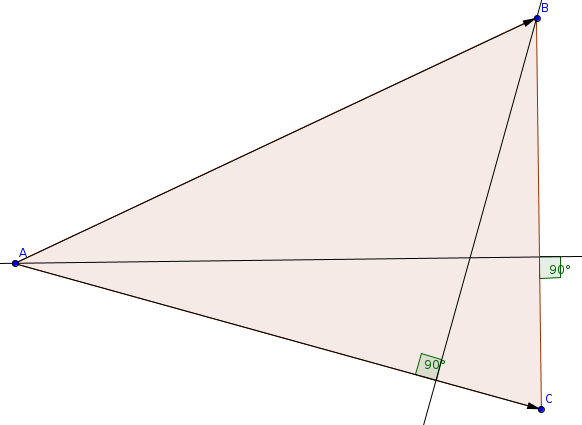
\includegraphics[width=0.49	\textwidth]{tri}
\caption{Kolmnurk ABC}
\label{fig:tri}
\end{wrapfigure}

Olgu kolmnurk \(ABC\) (joonis \ref{fig:tri}). Olgu punkt \(A\) koordinaatsüsteemi alguspunkt ja
vektorid \(\vec{AB}\) ja \(\vec{AC}\) vektorruumi baasiks. Nüüd on
võimalik kirjutada iga punkt selle kolmnurga tasandil nende vektorite
summana (võrrand \ref{eq:tri-1}).

\begin{equation} \label{eq:tri-1}
P' = A + u\vec{AB} + v\vec{AC}
\end{equation}

Kui \(u\) või \(v\) on väiksem kui null või suurem kui üks, asub punkt
kolmnurgast väljas. Kui punkt asub sirge \(BC\) kohal, on punkt
kolmnurgast väljas. Sirge \(BC\) võrrand on \(u + v = 1\), seega peab
punkti koordinaatide summa olema väiksem või võrdne ühega.

\subsubsection{Möller-Trumbore lähenemine}
Kiire lõikumise kolmnurgaga saab leida võrrandisüsteemist \ref{eq:tri-mt-1}.

\begin{equation} \label{eq:tri-mt-1}
\left\{
\begin{array}{l}
P' = P + t\vec s \\
P' = A + u\vec{AB} + v\vec{AC} \\
0 \leq u \leq 1 \\
0 \leq v \leq 1 \\
u + v \leq 1 \\
t > 0 
\end{array}
\right.
\end{equation}

\[P + t\vec s = A + u\vec{AB} + v\vec{AC}\]

\[u\vec{AB} + v\vec{AC} -t\vec s = (P - A)\]

\begin{equation} \label{eq:tri-mt-2}
u\vec{AB} + v\vec{AC} + t(-\vec s) = (P - A)
\end{equation}

Võrrand \ref{eq:tri-mt-2} on kolme tundmatuga lineaarvõrrandisüsteem,
mida on võimalik lahendada kolmerealise determinandiga. \cite{MT97}

\subsubsection{Waldi lähenemine}
\begin{wrapfigure}{R}{0.5\textwidth}
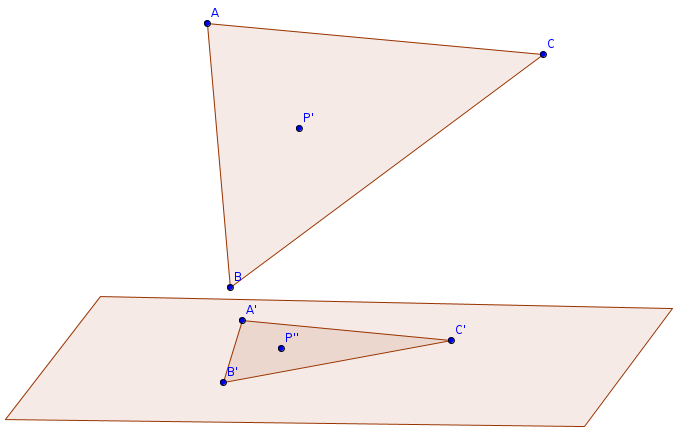
\includegraphics[width=0.49\textwidth]{tri-wald}
\caption{Projitseeritud kolmnurk}
\label{fig:tri-wald}
\end{wrapfigure}
Leida punkt \(P'\) kiire ja tasandi lõikumise võrrandist (võrrand
\ref{eq:plane3}), projitseerida kolmnurk ja leitud punkt mõnele koordinaatteljega
risti olevale tasandile (joonis \ref{fig:tri-wald}) ja lahendada võrrand \ref{eq:tri-1}. Tegurid, mis
ei sisalda punkti \(P'\) koordinaate, saab kolmnurkade töötlemisel välja
arvutada ja hiljem kasutada tippude koordinaatide asemel.
\cite[lk. 91]{wald::PhD}

\subsubsection{SSE4 skalaarkorrutis}
Koordinaate \(u\) ja \(v\) saab arvutada, projitseerides punkti \(P'\)
vastava koordinaadiga seotud külje tipust tõmmatud kõrgusele. Kolmemõõtmelises
ruumis võib kasutada ka kaugust tasandist, millel asub külg, millele see
kõrgus on tõmmatud, ja mis on kolmurgaga risti. Punkti ja tasandi vahelise
kauguse arvutamine nõuab skalaarkorrutise arvutamist, mis võtaks tavalisel
matemaatikaprotsessoril suhteliset kaua aega, kuid mille effektiivseks 
arvutamiseks on SSE4 käsustikus olemas eraldi masinkäsk \texttt{DPPS}.
\cite{TriSSE4}

\subsection{Kiire lõikumine keraga}
\begin{wrapfigure}{R}{0.45\textwidth}
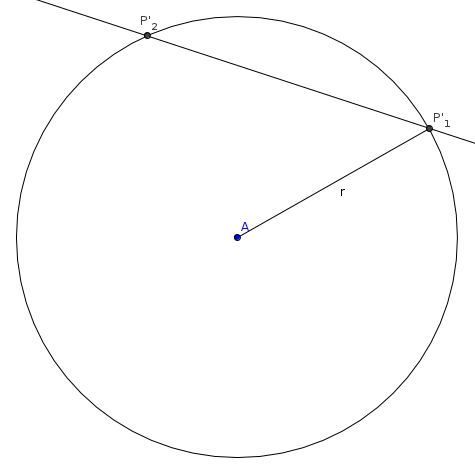
\includegraphics[width=0.4\textwidth]{sphere}
\caption{Kera}
\label{fig:sphere}
\end{wrapfigure}
Kera kõik punktid asuvad kera keskpunktist võrdsel kaugusel (joonis \ref{fig:sphere}).
\begin{equation} 
\left\{
\begin{array}{l}
(A - P')^2 = r^2 \\
P' = P + t\vec s
\end{array}
\right.
\end{equation}

\begin{equation} \label{eq:sphere1}
|\vec s|^2 t^2 + 2 t \vec s \cdot (A-P) + (A-P)^2 - r^2 = 0
\end{equation}

Kiire suunda tasub hoida ühikvektorina, sest hiljem läheb ühikpikkusega
suunda vaja peegeldusfunktsiooni väärtuse leidmisel, seega saab võrrandit
\ref{eq:sphere1} lihtustada taandatud ruutvõrrandiks.

\begin{equation} \label{eq:sphere2}
t^2 + 2 t \vec s \cdot (A-P) + (A-P)^2 - r^2 = 0
\end{equation}

Kui determinant on negatiivne, siis lõikepunktid puuduvad. Kui determinant
on null, siis on üks potensiaalne lõikekoht, ülejäänud juhtudel on kaks
potensiaalset lõikekohta.

\subsection{Kiire lõikumine silindriga}
Silinder otspunktidega \(A\) ja \(B\) ning raadiusega \(r\). Punkti \(P'\) kaugus sirgest \(AB\)
peab olema \(r\). Punkt \(P'\) ei tohi olla punktist \(A\) kaugemal kui \(B\) vektori \(\vec{AB}\)
sihis ja \(P'\) ei tohi olla punktist \(B\) kaugemal kui \(A\) vektori \(\vec{AB}\) sihis (võrrand \ref{eq:cyl-1}).

\begin{equation} \label{eq:cyl-1}
\left\{
\begin{array}{l}
\frac{\left(\vec{AB}\times\vec{AP'}\right)^2}{\vec{AB}^2} = r^2 \\
0\leq\vec{AB}\cdot\vec{AP'}\leq|\vec{AB}| \\
P' = P + t\vec s
\end{array}
\right.
\end{equation}

\begin{equation} \label{eq:cyl-2}
(\vec{AB}\times\vec s)^2 t^2 -2t(\vec{AB}\times\vec s)\cdot(\vec{AB}\times\vec{AP}) + (\vec{AB}\times\vec{AP})^2 - r^2(\vec{AB})^2 = 0
\end{equation}

Kui võrrandi \ref{eq:cyl-2} determinant on negatiivne, siis lõikepunktid
puuduvad. Kui determinant on null, siis on üks potensiaalne lõikekoht,
ülejäänud juhtudel on kaks potensiaalset lõikekohta. Lõikekohtadele
kehtivad võrrandisüsteemist \ref{eq:cyl-1} tulenevad piirangud.

\subsection{Ruutvõrrandi lahendamine}
Kera ja silindri lõikekohtade leidmiseks on vaja lahendada ruutvõrrand
parameetri \(t\) suhtes. Ujukomaarvude piiratuse tõttu võib tavapärane
lahend olla ebatäpne. Täpsemaks arvutamiseks peab lineaarliige ja ruutjuur
determinandist olema samamärgilised. Lisaks peab determinant olema arvutatud
kaks korda täpsema arvutüübiga, et täpsus säiliks. \cite{FP-quadratic}
Võrrand \ref{eq:quadratic} kirjeldab täpsemat ruutvõrrandi lahendivalemit.

\[ax^2+bx+c=0\]
\[q = -\frac 1 2 \left(b + sgn(b)\sqrt{b^2-4ac}\right)\]
\begin{equation}
\begin{array}{l l} \label{eq:quadratic}
x_1 = \frac q a; & x_2 = \frac c a : x_1 = \frac c a : \frac q a = \frac c q
\end{array}
\end{equation}

\section{Peegeldusfunktsioonid}
See alampeatükk kirjeldab erinevaid peegeldusfunktsioone. Kõiki
peegeldusfunktsioone võib omavahel kombineerida nii, et erinevate funktsioonide
peegelduskoefitsentide \(k\) summa oleks väiksem või võrdne ühega, muidu
iga põrge lisab süsteemi energiat.

\subsection{Lamberti peegeldufunktsioon}
\begin{figure}
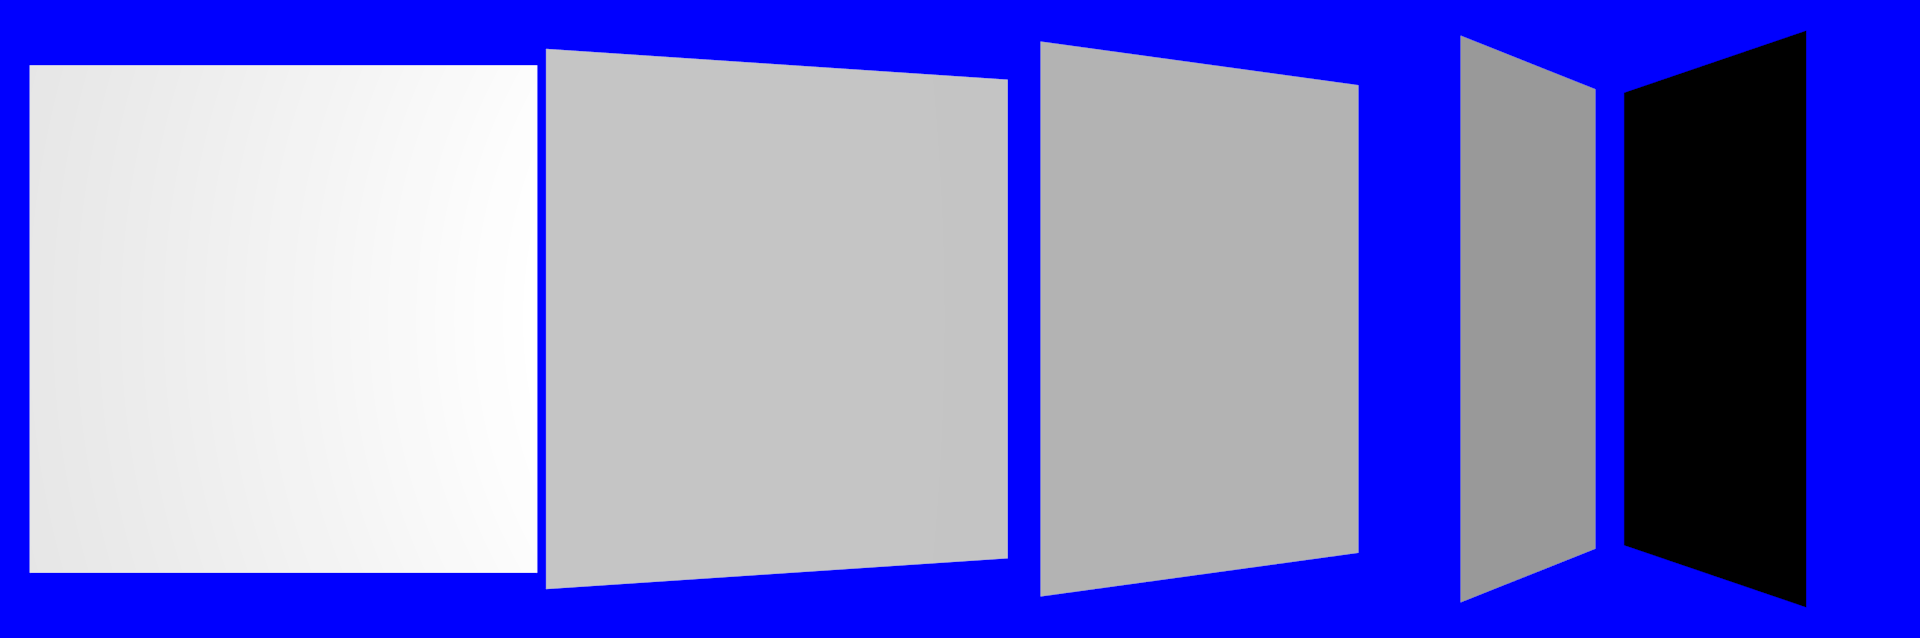
\includegraphics[width=\textwidth]{lambert}
\caption[Lamberti peegeldufunktsioon]{Lamberti peegeldufunktsioon.
Vasakult paremale valguse nurk \(0^\circ\), \(30^\circ\), \(45^\circ\),
\(60^\circ\) ja \(90^\circ\).}
\label{fig:lambert}
\end{figure}
Lamberti peegeldufunktsioon kirjeldab ideaalset matti keha, mille heledus
sõltub langeva valguse nurgast (joonis \ref{fig:lambert}, valem \ref{eq:lambert}).

\begin{equation} \label{eq:lambert}
f_r(\omega', \omega) = \frac k\pi \omega' \cdot \omega
\end{equation}

\subsection{Peegel} 
\label{subsec:peegel}
\begin{wrapfigure}{R}{0.5\textwidth}
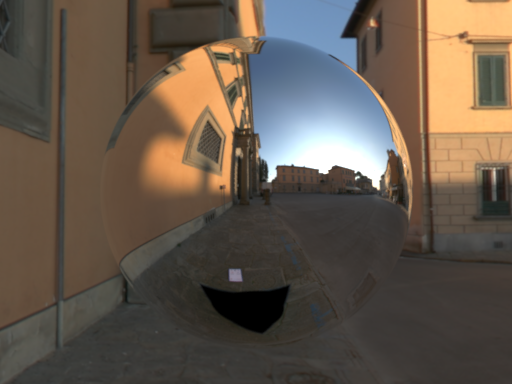
\includegraphics[width=0.499\textwidth]{mirror}
\caption[Peegel]{Peegel. Taust lehelt \url{http://gl.ict.usc.edu/Data/HighResProbes/}}
\label{fig:mirror}
\end{wrapfigure}

Peegli (joonis \ref{fig:mirror}) korral on sisenev ja väljuv valgus pinnanormaaliga sama nurga all.
Kuna pinnaga paralleelselt ei mõju footonile mingit jõudu, siis selle
kiiruse paralleelne komponent ei muutu (võrrand~\ref{eq:mirror-1}).
\begin{equation} \label{eq:mirror-1}
\omega_{||} = \omega'_{||} = \omega' - \omega'_{n} = \omega' -\vec n(\omega'\cdot\vec n)
\end{equation}

Kuna kiiruse paralleelne komponent jääb samaks, peab energia jäävuse
seaduse järgi kiiruse normaalisuunalise komponendi absoluutväärtus jääma
samaks. Valgus eemaldub pinnast, seega peab komponendi märk olema vastupidine
endisele (võrrand~\ref{eq:mirror_2}).

\begin{equation} \label{eq:mirror_2}
\omega_n = -\omega'_n = -\vec n(\omega'\cdot\vec n)
\end{equation}

\begin{minipage}{0.5\textwidth}
\[\omega = \omega_{||} + \omega_n = \omega' - 2\vec n(\omega'\cdot\vec n)\]
\end{minipage}

\[f_r(\omega', \omega) = \left\{\begin{array}{l l} k_s & \quad \text{kui} ~ -[\omega'-2\vec n(\omega'\cdot\vec n)] = \omega \\ 0 \end{array} \right. \]

\subsection{Phongi udune peegel}
\begin{figure}[h]
\centering
\subfloat[\(\alpha=50\)]{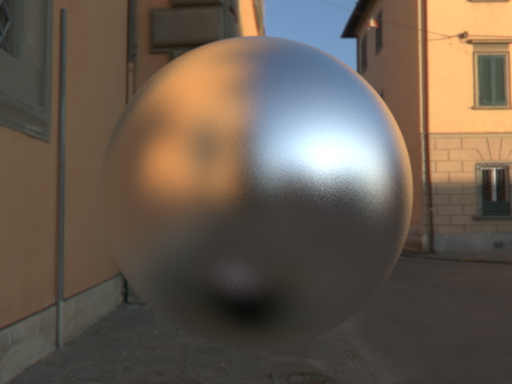
\includegraphics[width=0.25\textwidth]{phong-50}}
\subfloat[\(\alpha=100\)]{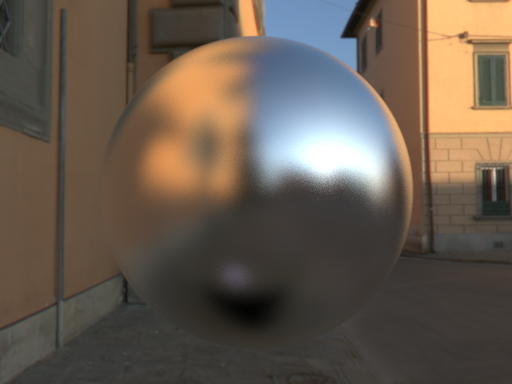
\includegraphics[width=0.25\textwidth]{phong-100}}
\subfloat[\(\alpha=200\)]{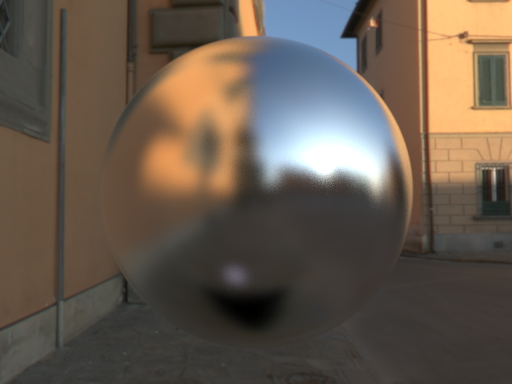
\includegraphics[width=0.25\textwidth]{phong-200}}
\subfloat[\(\alpha=8000\)]{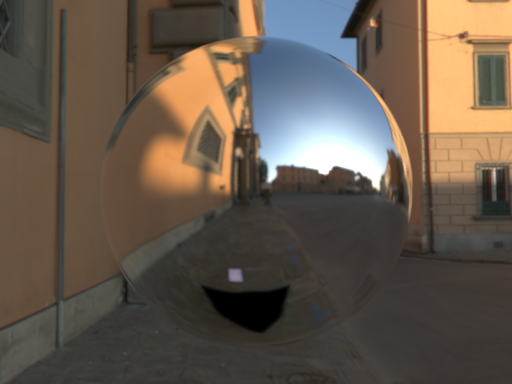
\includegraphics[width=0.25\textwidth]{phong-8000}}
\caption[Phongi udune peegel]{Phongi udune peegel. Taust lehelt \url{http://gl.ict.usc.edu/Data/HighResProbes/}}
\label{fig:phong}
\vspace{100pt}
\end{figure}
Phongi udune peegel (joonis \ref{fig:phong}) kirjeldab kehi, mille pinnakaredused hajutavad
peegelduvat valgust. Parameeter \(\alpha\) kirjeldab kui kitsas on peegelduva
valguse koonus. Kui \(\alpha\) läheneb lõpmatusele, sarnaneb tulemus
osas \ref{subsec:peegel} kirjeldatuga.

\begin{equation}
f_r(\omega', \omega) = \frac{k(\alpha+2)}{2\pi}\{[\omega'-2\vec n(\omega'\cdot\vec n)]\cdot\omega\}^\alpha
\end{equation}

\section{Joonistuskiiruse suurendamine}
Isegi kui kasutada kõige effektiivsemaid algoritme, optimeerida nii
masinkoodi kui ka mälus paiknemist ja vähendada mälukasutust, on
kiirtejälitus aeglane võrreldes teiste ilmestusmeetoditega.

\subsection{Paralleeltöötlus}
Kiirtejälituses ja ka arvutigraafikas üldiselt ei sõltu pildipiksli
väärtus teistest pikslitest. Seega on võimalik piisava arvutusvõimsuse
olemasolul arvutada kõik pikslid paralleelselt.

\subsubsection{Paralleeltöötluse käsustikud}
Mõned käsustikud (nt. Inteli x86 protsessorites MMX, SSE ja AVX) suudavad
sooritada korraga tervel andmehulgal sama operatsiooni ligikaudselt ajaga,
mis kulub tavalise käsustikuga ühe elemendi töötlemiseks. Eelmainitud
käsustikest opereerivad uju\-koma\-arvudega ainult SSE (\textit{Streaming
SIMD Extensions}) ja AVX (\textit{Advanced Vector Extensions}), mis 
töötlevad vastavalt nelja ja kaheksa 32-bitise või kahe ja nelja 64-bitise
ujukomaarvuga korraga. Registri laiusest olenevalt on võimalik töödelda
mitut kiirt korraga. Samas ei ole see ilma probleemideta, sest kumerad
pinnad hajutavad valgust ja peale paari põrget võib kiirte vaheline kaugus
olla liiga suur, et selline paralleeltöötlus ära tasuks. Teine võimalus
on kasutada paralleeltöötluse käsustikke vektoritega arvutamise kiirendamiseks.
See ei paku nii suurt kiirusetõusu kui esimene variant kuid töötab alati.

\subsubsection{Lõimtöötlus}
Kuna kõikidel uutel protsessoritel on mitu tuuma on võimalik leida mitme
piksli väärtus korraga. Ainsaks takistuseks on, et lõimtöötluse realisatsioonid
on eri operatsiooni\-süstee\-mides erinevad, ainult UNIXi derivaatidel on
UNIXi spetsifikatsioonist tulenev \texttt{pthread}i toetus, mis puudub
Windowsil. Lahenduseks on GCC (GNU Compiler Collection) ja Microsofti
Visual Studio poolt toetatud OpenMP (Open MultiProcessing) spetsifikatsioon.
OpenMP plussiks on veel ka lihtne kasutamine ja automaatne skaleerimine,
mis tähendab, et OpenMP loob ise vajaliku arvu lõimi vastavalt tuumade
arvule. Kiirusetõus on võrdelises seoses kasutatavate tuumade arvuga.

\subsubsection{Graafikaprotsessoril arvutamine}
Graafikaprotsessorid on põhimõtteliselt väga võimsad paralleelsed
ujukomaprotsessorid. Graafikakaartide tootjad on lisanud graafikakonveieri
võimaluse käivitada graafikakaardil oma koodi algul materjalide kirjeldamiseks
kuid hiljem ka suvalise koodi käivitamiseks.

\subsection{Optimeerimine}
Lisaks kõige kangemate kompilaatori optimeeringute sisselülitamise saab
programmi kiiremaks, kui arvutada varem välja väärtused, mis sõltuvad
ainult sisendandmetest ja mida läheb hiljem vaja, nagu näiteks planaarsete
kujundite pinnanormaalid ning kera ja silindri raadiuste ruudud. Samuti
saab mitu sama arvuga jagamist ümber kirjutada üheks jagamiseks ja mitmeks
korrutamiseks. Trigonomeetrilised funktsioonid ja astmefunktsioonid on
aeglased, neid tasub vältida nii palju kui võimalik.

\subsubsection{Vektori normeerimine}
Vektori normeerimiseks on vaja vektor jagada selle pikkusega (valem \ref{eq:vec-1}).

\[\vec v = (x; y; z)\]
\begin{equation} \label{eq:vec-1}
|\vec v| = \sqrt{x^2 + y^2 + z^2}
\end{equation}

SSE käsustikus on ligikaudse ruutjuure pöördarvu (\(\frac 1 {\sqrt x} = x^{-\frac12}\)) leidmise käsk
\texttt{RSQRTSS}, mis leiab avaldise väärtuse esimesest elemendist, ja
käsk \texttt{RSQRTPS}, mis leiab väärtuse kõigist neljast elemendist.
Nende käskude maksimaalne viga on \(\leq 1.5 \cdot 2^{-12}\). Kui kasutada Newtoni
meetodi ühte iteratsiooni on võimalik muuta viga sama suureks kui 32-bitise
ujukomaarvu viga. Võrrand \ref{eq:vec-2} on Newtoni meetodi iteratsiooni
üldkuju.

\begin{equation} \label{eq:vec-2}
x_{n+1} = x_n - \frac {f(x_n)}{f'(x_n)}
\end{equation}

Võrrand \ref{eq:vec-3} näitab funktsiooni, mille nullkohta on vaja leida.

\[x = \frac 1 {\sqrt a}\]
\[\frac 1{x^2} = a\]
\begin{equation} \label{eq:vec-3}
f(x) = \frac 1{x^2} - a = 0
\end{equation}
\begin{equation} \label{eq:vec-4}
f'(x) = -\frac 2{x^3}
\end{equation}

Asendades võrrandid \ref{eq:vec-3} ja \ref{eq:vec-4} võrrandisse \ref{eq:vec-2},
on tulemuseks võrrand \ref{eq:vec-5}, mis kasutades koos vastava masinkäsuga
on kiirem kui matemaatikateegi sarnased funktsioonid.

\begin{equation} \label{eq:vec-5}
x_{n+1} = x_n - \frac {\frac 1{x_n^2} - a}{-\frac 2{x_n^3}} = 0.5x_n(2 + 1 - ax_n^2) = 0.5x_n(3-ax_n^2)
\end{equation}

\subsection{Ruumi jaotamine puudesse}
Kiirtejälituse kiirust saab tõsta vähendades arvutatavate lõikumiste arvu.
Selleks kasutatakse tavaliselt mõnda kahendpuu vormi.

\subsubsection{Kaheksapuu}
\begin{wrapfigure}{R}{0.45\textwidth}
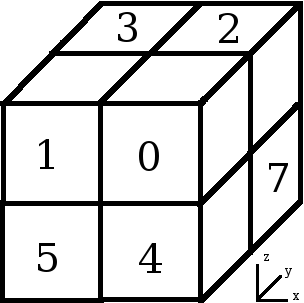
\includegraphics[width=0.4\textwidth]{octree}
\caption{Alampuude nummerdamine uurimistööga kaasas olevas kiirtejälitajas}
\label{fig:octree}
\end{wrapfigure}
Kaheksapuu (ing. k. \textit{Octree}) jaotab igal astmel ruumi kaheksaks
osaks (joonis \ref{fig:octree}). Igas oktandis asetsevad kujundid asuvad selles alampuus ja kujundid,
mis ei mahu alapuudesse, asetsevad madalaimas võimalikus tipus. Kaheksapuu
läbi käimiseks on vaja iga oktandi korral leida, kas kiir seda läbib, ning
leida sealt lähim pind.

\subsubsection{kD-puu}
kD-puu (ing. k. \textit{kD-tree}) on kahendpuu, mis jaotab n-mõõtmelise
ruumi teljega risti oleva hüpertasandiga kaheks osaks. Optimaalse kD-puu
konstrueerimiseks kasutatakse pindalaheuristikat. Iga võimaliku hüpertasandi
arvutatkse sellest kohast poolitamise hind. Kui poolitamise hind on suurem
kui mittepoolitamise hind, lõpetatakse poolitamine. Poolitamise hind on
mõlema alampuu hindade summa ja võrrand \ref{eq:SAH} näitab alampuu 
läbimise hinda.

\begin{equation} \label{eq:SAH}
C = C_t + S \cdot n \cdot C_i
\end{equation}
\begin{itemize}
\item[\(\mathbf{C_t}\)] kD-puu läbimise hind
\item[\(\mathbf{S}\)] alampuu pindala
\item[\(\mathbf{n}\)] kujundite arv alampuus
\item[\(\mathbf{C_i}\)] kiire kujunditega lõikumiste uurimise hind
\end{itemize}

\chapter*{Kokkuvõte}
\addcontentsline{toc}{chapter}{Kokkuvõte}
Uurimistöö eesmärgiks oli anda ülevaade ja kiirtejälituse põhiprotsesside
suhtes sai eesmärk täidetud. 

Kirjeldati:
\begin{itemize}
\item valguse füüsikalist mudelit,
\item Monte Carlo meetodit multidimensionaalsete integraalide arvutamiseks,
\item kiirte lõikumist erinevate kolmemõõtmeliste kujunditega,
\item erinevaid peegeldusfunktsioone ja
\item kolmemõõtmelise ruumi jaotamist kahendpuusse.
\end{itemize}

Uurimistöös toodi välja ka erinevad kiirtejälituse kiiruse tõstmise
võimalused, millest on kasutatud näidisprogrammis kõiki peale
graafikaprotsessoril arvutamist.

% Kasutatud materjalid
\renewcommand\bibname{Kasutatud materjalid}
\bibliographystyle{apacite}
\bibliography{paper}

\appendix
%\chapter{Radiomeetria mõisted}
%\begin{description}
%\item[Kiirgusvoog] (ing. k. \textit{radiant flux}) on energiahulk, mille kiirgus kannab ajaühikus läbi pinna.
%\item[Kiiritustihedus] (ing. k. \textit{irradiance}) iseloomustab ruumi- ja mittepunktvalgusallikate kiiratud valgust.
%\item[Kirkus] (ing. k. \textit{radiance}) nimetatakse pinnale langevat kiirgusvoogu.
%\end{description}
\chapter{Kiirtejälitaja} \label{chap:download}
Uurimistöö raames valmis programm, mis kasutab uurimistöös kirjeldatud
algoritme ja ideid. Programmi suhteliselt suure mahu tõttu ei ole võimalik
seda siin ära tuua. Programmi lähtekood on saadaval \texttt{git}i varamust
aadressil \url{https://github.com/andreasots/raytracer}. Programmi kompileerimiseks
on vaja Single UNIX spetsifikatsioonile vastavat operatsioonisüsteemi,
vastavalt operatsioonisüsteemile kas DirectX (Windows), X11 (Unix) või
Cocoa (MacOS) teeke ja päiseid, OpenEXR teeki ning selle päiseid ja
viimast C++ versiooni toetavat kompilaatorit. Lähtekoodiga on kaasas
Code::Blocksi projektifail.

\chapter*{Resümee}
Kiirtejälitus on arvutigraafika algoritm, mis suudab luua realistlikuma
kujutise kui rohkem kasutatud rasteriseerimine. Uurimistöös on kirjeldatud
kiirtejälituse alussüsteeme nagu näiteks:
\begin{itemize}
\item valguse füüsikalist mudel,
\item Monte Carlo meetod multidimensionaalsete integraalide arvutamiseks,
\item kiirte lõikumine erinevate kolmemõõtmeliste kujunditega,
\item erinevad peegeldusfunktsioonid ja
\item kolmemõõtmelise ruumi jaotamine kahendpuusse.
\end{itemize}

Uurimistöö raames kirjutati lihtne kiirtejälitaja, mis kasutab uurimistöös
kirjeldatud meetodeid.

\chapter*{Abstract}
Raytracing is a computer graphics algorithm that can create more realistic
image than more commonly used rasterisation. This research paper covers
the basics of raytracing such as:
\begin{itemize}
\item basic radiometry,
\item Monte Carlo method for evaluation of multidimentional integrals,
\item ray-object intersections,
\item bidirectional reflectance distribution functions (BRDF) and
\item space partitioning trees.
\end{itemize}

The research paper also contains a simple reference raytracer which uses
the methods described in the paper.

\chapter*{Kinnitusleht}
Kinnitan, et
\begin{itemize}
\item koostasin uurimistöö iseseisvalt. Kõigile töös kasutatud teiste autorite töödele ja
andmeallikatele on viidatud;
\item olen teadlik, et uurimistööd ei edastata teistele tulu teenimise eesmärgil ega jagata
teadlikult plagieerimiseks.
\end{itemize}

\flushleft
~\\\dotfill\\
kuupäev / nimi / allkiri

~\\

Tunnistan lõputöö kaitsmisvalmiks.

Juhendajad

\flushleft
~\\\dotfill\\
kuupäev / nimi / allkiri

\flushleft
~\\\dotfill\\
kuupäev / nimi / allkiri

\end{document}
